\newpage
\begin{tcolorbox}[breakable, enhanced jigsaw]
{\color{blue}
2.2) Una pastilla de silicio compuesta por dos materiales tipo \textit{n} se encuentra en equilibrio térmico. Las regiones presentan concentraciones de donantes \(N_{D1}\) y \(N_{D2}\).}
\end{tcolorbox}
Tanto la corriente de arrastre como la corriente de difusión son iguales y opuestas en cada punto, por lo que la corriente total en equilibrio térmico para los electrones será:
\begin{align}
    J_{a,n} &= q\cdot n(x)\cdot E(x)\cdot \mu_n,\\
    J_{d,n} &= q\cdot D_n \frac{dn(x)}{dx}.
\end{align}
Por lo que tendremos que la corriente total es:
\begin{align}
    J_{n} &= J_{a,n} + J_{d,n} = 0,\\
    J_{a,n} &= -J_{d,n},\\
    q\cdot n(x)\cdot E(x)\cdot \mu_n &= -q\cdot D_n \frac{dn(x)}{dx}.
\end{align}
Dado que el \textbf{campo eléctrico} es \(E(x)=-\frac{dV(x)}{dx}\), se tiene que: 
\begin{align}
    -n(x)\cdot \mu_n \frac{dV(x)}{dx} &= -D_n \frac{dn(x)}{dx},\\
    n(x)\cdot \mu_n\, dV(x) &= D_n\, dn(x).
\end{align}
Luego, tomando en cuenta la ecuación de Einstein:
\begin{align}
    \frac{D_n}{\mu_n} &= \frac{k_B T}{q} = V_T,
\end{align}
entonces se tendrá que:
\begin{align}
    dV(x) &= V_T \frac{dn(x)}{n(x)},\\
    dV(x) &= \frac{k_B T}{q}\,\frac{dn(x)}{n(x)}.
\end{align}
Con lo que, integrando sobre los puntos dados en la figura:
\begin{figure}
    \centering
    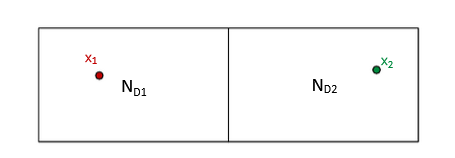
\includegraphics[scale=1]{img/P1_3.png}
    \caption{Pastilla \(n\!-\!n\): dos regiones con dopajes \(N_{D1}\), \(N_{D2}\); puntos \(x_1\), \(x_2\) para evaluar \(V\). El gradiente de dopaje induce un campo interno.}
\end{figure}
tenemos que:
\begin{align}
    \int_{V(x_1)}^{V(x_2)} dV(x) &= V_T \int_{n(x_1)}^{n(x_2)} \frac{dn(x)}{n(x)},
\end{align}
con lo que finalmente se obtiene:
\begin{align}
    V(x_2)-V(x_1) &= V_T \ln\!\frac{n(x_2)}{n(x_1)}.
\end{align}
Con lo que las diferentes zonas serán:
\begin{itemize}
    \item \(N_{D1}>N_{D2}\) \(\Rightarrow\) \(n(x_1)>n(x_2)\) \(\Rightarrow\) \(V(x_2)-V(x_1)<0\) \(\Rightarrow\) \(V(x_2)<V(x_1)\).
    \item \(N_{D1}<N_{D2}\) \(\Rightarrow\) \(n(x_2)>n(x_1)\) \(\Rightarrow\) \(V(x_2)-V(x_1)>0\) \(\Rightarrow\) \(V(x_2)>V(x_1)\).
    \item \(N_{D1}=N_{D2}\) \(\Rightarrow\) \(n(x_1)=n(x_2)\) \(\Rightarrow\) \(V(x_2)-V(x_1)=0\) \(\Rightarrow\) \(V(x_2)=V(x_1)\).
    \item Si \(V(x_1)=0\) \(\Rightarrow\) \(\displaystyle V(x_2)=V_T \ln\!\frac{N_{D2}}{N_{D1}}\) \text{ (con } \(x_1\) en la región \(N_{D1}\) y \(x_2\) en \(N_{D2}\)\text{)}.
\end{itemize}
\begin{itemize}
    \item  \textbf{Zona más dopada vs. menos dopada} (\(N_{D1}>N_{D2}\)): La región con mayor concentración de donantes tiene más electrones libres que tienden a difundirse hacia la región menos dopada, creando un campo eléctrico interno que establece una barrera energética. El potencial resulta menor en la zona más dopada (\(V(x_2)<V(x_1)\)), equilibrando la difusión con la deriva eléctrica en condiciones de equilibrio térmico.
\item  \textbf{Zona menos dopada vs. más dopada} (\(N_{D1}<N_{D2}\)): En este caso inverso, la difusión neta ocurre desde la región \(x_2\) hacia \(x_1\), formando un campo eléctrico que apunta desde la región de mayor potencial hacia la de menor potencial. El resultado es que el potencial es mayor en la zona originalmente menos dopada (\(V(x_2)>V(x_1)\)).
\item \textbf{Zona de dopaje uniforme} (\(N_{D1}=N_{D2}\)): Cuando no existe gradiente de concentración, no hay fuerza de difusión neta, por lo que el potencial permanece constante a través de todo el material (\(V(x_2)=V(x_1)\)). No se forma campo eléctrico interno y el material se comporta como un semiconductor homogéneo sin barreras energéticas internas.
\item \textbf{Relación logarítmica del potencial}: La diferencia de potencial \(V(x_2)=V_T \ln\!\frac{N_{D2}}{N_{D1}}\) surge de la estadística de Fermi-Dirac y la condición de equilibrio térmico, donde \(V_T = \frac{k_B T}{q}\) es el potencial térmico (\(\approx 26\) mV a temperatura ambiente). La dependencia logarítmica refleja la naturaleza exponencial de la distribución de portadores en función de la energía, estableciendo que el potencial es mayor en la zona de menor concentración de donantes.
\end{itemize}

\begin{tcolorbox}[breakable, enhanced jigsaw]
    {\color{blue}
2.1) Se dopa ahora el lado derecho de la pastilla con impurezas aceptoras, de modo que \(N_A>N_D\). Obtenga el campo eléctrico máximo y bosqueje un diagrama de bandas de energía.}
\end{tcolorbox}

Dado que ahora el lado derecho se dopa tipo \(p\) (\(N_A>N_D\)) \(\Rightarrow\) unión \(p\!-\!n\). Se pide \(E_{\max}\) y dibujar las bandas de energía en equilibrio, se dibuja lo siguiente:
\begin{figure}
    \centering
    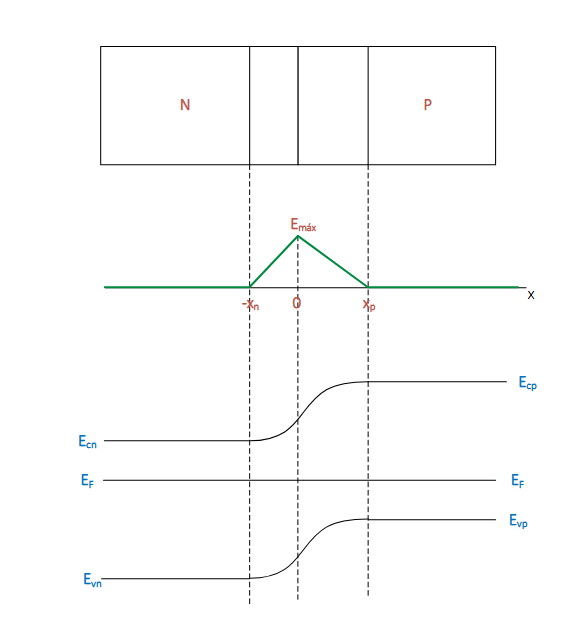
\includegraphics[scale=0.8]{img/P1_5.png}
    \caption{Bandas en unión \(p\!-\!n\) en equilibrio: \(E_C\), \(E_V\), \(E_F\) con doblamiento en la región de agotamiento (barrera \(V_0\)). \(E_{\max}\) en la interfaz de máxima curvatura.}
\end{figure}

\begin{tcolorbox}[breakable, enhanced jigsaw]
{\color{blue}
2.3) Determine y grafique la concentración de portadores a ambos lados de la pastilla, el diagrama de concentraciones, el campo eléctrico en la zona de transición, el potencial eléctrico a lo largo de la pastilla.}
\end{tcolorbox}

Las ecuaciones que usaremos son la \textit{ley de acción de masas} y la \textit{neutralidad de carga}, las cuales vienen dadas por:
\begin{align}
n\,p &= n_i^{2},\\
n + N_D &= p + N_A.
\end{align}
Por enunciado, tenemos los siguientes datos: \(n_i = 10^{10} \,\text{cm}^{-3}\), \(N_{D1} = 10^{16} \,\text{cm}^{-3}\) y, dado que no se menciona dopaje aceptor, \(N_{A1} = 0 \,\text{cm}^{-3}\). Por lo que finalmente se tiene 
\begin{align}
n\,p &= n_i^{2},\\
n &= p + N_D.
\end{align}
Luego, tenemos que:
\begin{align}
    n= \frac{n_i^2}{n} + N_{D},\\
    n^2 - N_D\, n - n_i^2 &= 0.
\end{align}
Con lo que tenemos una ecuación cuadrática, la cual se puede resolver con la fórmula general:
\begin{align}
    n_{1,2}=\frac{-(-N_D)\pm\sqrt{N_D^{2}-4(1)(-n_i^{2})}}{2(1)}.
\end{align}
Notamos que, evidentemente, \(N_D^2 \gg 4n_i^2\) (p.\ ej., \(10^{32}\gg 4\cdot 10^{20}\)), por lo que se puede aproximar la solución como:
\begin{align}
    n &\simeq \frac{N_D+\sqrt{N_D^2}}{2} \simeq N_D = 10^{16}\,\text{cm}^{-3}.
\end{align}
Por lo que la concentración de huecos resulta:
\begin{align}
    p=\frac{n_i^2}{n}=\frac{10^{20}}{10^{16}}=10^{4}\,\text{cm}^{-3}.
\end{align}

Ahora calculamos las concentraciones del otro material, usando las mismas dos ecuaciones:
\begin{align}
n\,p &= n_i^{2},\\
n + N_A &= p + N_D.
\end{align}
Dados los datos entregados, tenemos \(n_i = 1{,}12\times 10^{10}\,\text{cm}^{-3}\), \(N_{D2}=10^{14}\,\text{cm}^{-3}\) y \(N_A=10^{17}\,\text{cm}^{-3}\). Entonces:
\begin{align}
n\,p &= n_i^{2},\\
n + N_A &= p + N_D.
\end{align}
De la primera ecuación despejamos \(n\) y lo reemplazamos en la segunda:
\begin{align}
    \frac{n_i^2}{p}+N_A &= p+N_D,\\
    p^2 + (N_D-N_A)\,p - n_i^2 &= 0.
\end{align}
Como \(N_A \gg N_D\), es razonable aproximar \(N_D-N_A \approx -N_A\). Entonces:
\begin{align}
    p^2 - N_A\, p - n_i^2 &= 0,
\end{align}
con solución:
\begin{align}
    p_{1,2}=\frac{-(-N_A)\pm\sqrt{N_A^{2}-4(1)(-n_i^{2})}}{2(1)}.
\end{align}
Dado que \(N_A^2 \gg 4n_i^2\) (p.\ ej., \(10^{34}\gg 4\cdot 10^{20}\)), se obtiene:
\begin{align}
    p &\simeq \frac{N_A+\sqrt{N_A^2}}{2} \simeq N_A = 10^{17}\,\text{cm}^{-3}.
\end{align}
La concentración de electrones vale:
\begin{align}
    n=\frac{n_i^2}{p}=\frac{(1{,}12\times 10^{10})^2}{10^{17}}
    \simeq 1{,}25\times 10^{3}\,\text{cm}^{-3}\approx 10^{3}\,\text{cm}^{-3}.
\end{align}
Luego, podemos dibujar el diagrama de concentraciones:
\begin{figure}
    \centering
    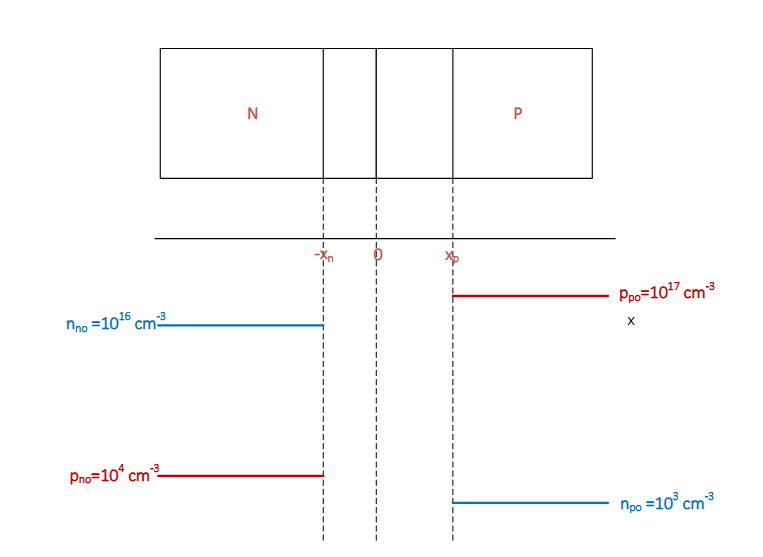
\includegraphics[scale=0.8]{img/P1_6.png}
    \caption{Concentraciones en equilibrio para unión \(p\!-\!n\): en N, \(n_{n0}\gg p_{n0}\); en P, \(p_{p0}\gg n_{p0}\). En la zona de agotamiento, las mayorías disminuyen y las minorías aumentan levemente.}
\end{figure}
Buscamos determinar el campo eléctrico máximo. Primero hallamos \(V_0\) (barrera de potencial) y
\(L\) (ancho total de la zona de agotamiento); la barrera de potencial viene dada por:
\begin{align}
V_0 &= V_T \ln\!\left(\frac{p_{p0}}{p_{n0}}\right),\\
V_0 &= 0{,}0258~\text{V}\,\ln\!\left(\frac{10^{17}}{10^{4}}\right) = 0{,}77~\text{V}.
\end{align}
El valor positivo indica que \(V_p>V_n\) bajo la convención adoptada. La longitud de la zona de agotamiento \(L\) viene dada por
\begin{align}
L&=\sqrt{\frac{2\,|V_0|\,\varepsilon_s}{q}\!\left(\frac{1}{N_A}+\frac{1}{N_D}\right)},\\
% En la expresión anterior, \(N_D\) corresponde al lado n del semiconductor (aquí usamos \(N_D=N_{D1}=10^{16}\,\text{cm}^{-3}\)).
L &= \sqrt{\frac{2(0{,}77)\times 10^{-12}}{1{,}6\times 10^{-19}}
\left(\frac{1}{10^{17}}+\frac{1}{10^{16}}\right)}~\text{cm} \\
  &= 3{,}254\times 10^{-5}~\text{cm}.
\end{align}
Con lo que tendremos que el \textbf{campo eléctrico} máximo será:
\begin{align}
E_{\max}&=\frac{2\,|V_0|}{L}
= \frac{2(0{,}77~\text{V})}{3{,}254\times 10^{-5}~\text{cm}}
= 4{,}73286\times 10^{4}\;\frac{\text{V}}{\text{cm}}.
\end{align}
Finalmente, se tiene que:
\begin{equation}
\boxed{\,E_{\max}\approx 4{,}7329\times 10^{4}\; \text{V/cm}\,}
\end{equation}
Gráficamente se observa:
\begin{figure}
    \centering
    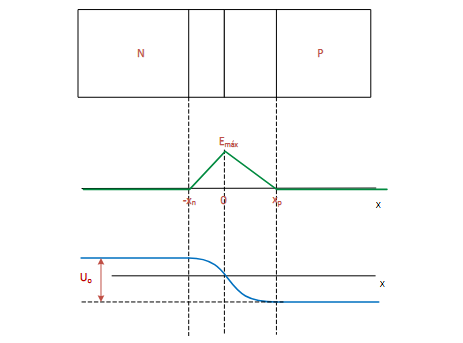
\includegraphics[scale=1]{img/P1_7.png}
    \caption{Campo eléctrico en la unión \(p\!-\!n\): triangular en la región de agotamiento, con máximo \(E_{\max}\) en el centro; fuera de ella es prácticamente nulo.}
\end{figure}
\begin{figure}
    \centering
    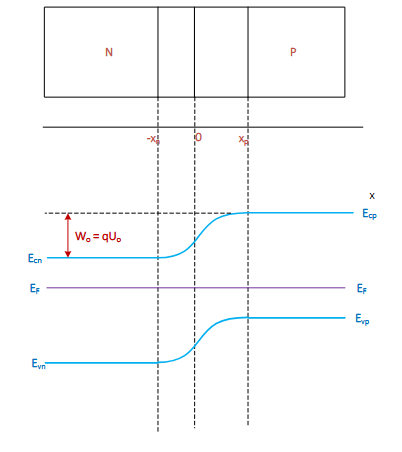
\includegraphics[scale=1]{img/P1_8.png}
    \caption{Potencial eléctrico \(V(x)\) y bandas: salto \(qV_0\) entre regiones N y P; el nivel de Fermi \(E_F\) es plano en equilibrio.}
\end{figure}
Donde tenemos que 
\begin{align}
W_0 &= q\,V_0,\\
    &= q\,(0{,}77~\text{V}) \simeq 0{,}77~\text{eV}.
\end{align}
Como la energía de barrera es una magnitud,
\begin{equation}
\boxed{\,W_0 = |qV_0| = |V_0|~\text{eV} = 0{,}77~\text{eV}\, }.
\end{equation}
